\chapter{Niet-coderende RNA's en posttranscriptionele regulatie}\label{ch:b3:rna-regulation}

In 1990 probeerden twee plantenbiologen petunia's dieper paars te
maken door ze extra kopieën van het gen voor het pigmentenzym te
geven. Bijna de helft van de transgene planten kwam er wit uit, of
paars met witte sectoren: het toegevoegde gen had de eigen kopie van
de plant samen met zichzelf uitgeschakeld. Acht jaar later vonden twee
wormgenetici die RNA in \emph{Caenorhabditis elegans} injecteerden dat
een dubbelstrengs RNA dat bij een spiergen paste dat gen uitschakelde,
in de geïnjecteerde worm en in haar nageslacht, veel krachtiger dan
elk van beide strengen afzonderlijk. De twee raadsels hadden één
antwoord: cellen bezitten een machinerie die met korte RNA's RNA's met
een passende sequentie opspoort en uitschakelt. Die machinerie, en de
bredere wereld van regulatie die een boodschapper-RNA ondergaat nadat
het is afgeschreven --- hoe het wordt gesplitst, waarheen het wordt
gestuurd, hoe lang het leeft, of het wordt vertaald --- is het
onderwerp van dit hoofdstuk. Het boek van jaar 1 behandelde het gen
als een eenheid die aan of uit staat bij haar promotor; hier wordt het
transcript zelf het voorwerp van sturing.

\section{De RNA-telling van een cel}

\begin{definition}[Niet-coderend RNA]\label{def:b3:rna-regulation:ncrna}
\index{niet-coderend RNA}\index{microRNA}\index{siRNA}\index{piRNA}\index{lang niet-coderend RNA}\index{klein nucleair RNA}
Een \emph{niet-coderend RNA} (ncRNA) is een transcript dat als RNA
werkt en niet als matrijs voor een eiwit. Behalve de ribosomale en
transfer-RNA's van de translatie en de \emph{kleine nucleaire RNA's}
(snRNA's) van het spliceosoom bevat een eukaryote cel:
\emph{microRNA's} (miRNA's), \numrange{21}{23} nucleotiden, geknipt uit
haarspelden in de eigen transcripten van de cel en sturend bij de
onderdrukking van deels complementaire boodschappers; \emph{kleine
interfererende RNA's} (siRNA's), even lang, geknipt uit lang
dubbelstrengs RNA en sturend bij de knip van volmaakt passende
doelwitten; \emph{Piwi-interagerende RNA's} (\omterm{def:b3:rna-regulation:pirna}{piRNA's}),
\numrange{26}{31} nucleotiden, werkzaam in de kiembaan tegen
transposons; kleine nucleolaire RNA's die de modificatie van rRNA
sturen; en \emph{lange niet-coderende RNA's} (lncRNA's), transcripten
langer dan \qty{200}{nt} zonder open leesraam van betekenis, waarvan
\emph{\omterm{def:b3:chromatin-epigenetics:x-inactivation}{Xist}} uit \cref{ch:b3:chromatin-epigenetics} het best begrepen
is. Eiwitcoderende exons beslaan ongeveer \qty{1.5}{\%} van het
menselijk genoom; een groot deel van de rest wordt ooit in een of
andere cel afgeschreven, maar hoeveel van die transcriptie functioneel
is, is een open vraag.
\end{definition}

\begin{remark}[Overvloed is geen functie]\label{rem:b3:rna-regulation:function}
Een transcript kan aantoonbaar zijn omdat het polymerase lekt, niet
omdat het RNA iets doet; de meeste lncRNA's komen in minder dan één
kopie per cel voor, zijn slecht geconserveerd en zijn bij deletie
misbaar. De toets op functie is genetisch: een fenotype wanneer het
RNA, en niet enkel zijn DNA, wordt weggehaald. \emph{\omterm{def:b3:chromatin-epigenetics:x-inactivation}{Xist}}, de
miRNA's en de \omterm{def:b3:rna-regulation:pirna}{piRNA's} doorstaan haar overtuigend; van de tienduizenden
geannoteerde lncRNA's hebben er tot nu toe enkele honderden dat gedaan.
\end{remark}

\section{RNA-interferentie en de microRNA's}

\begin{definition}[RNA-interferentie]\label{def:b3:rna-regulation:rnai}
\index{RNA-interferentie}\index{Dicer}\index{Argonaute}\index{RISC}
\emph{RNA-interferentie} (RNAi) is de sequentiespecifieke
uitschakeling van een gen door een klein RNA dat van dubbelstrengs RNA
afkomstig is. Het enzym \emph{Dicer}, een RNase III, knipt lang
dubbelstrengs RNA in duplexen van \numrange{21}{23} nucleotiden met
3$'$-overhangen van twee nucleotiden; van elke duplex wordt één
streng, de gids, in een \emph{Argonaute}-eiwit geladen, waarmee het
\emph{RNA-geïnduceerde uitschakelingscomplex} (RISC) ontstaat. De gids
paart met een complementair doel-RNA, en het endonucleasedomein van
Argonaute knipt het doelwit tegenover de nucleotiden 10 en 11 van de
gids; het geknipte RNA wordt daarna afgebroken en het RISC komt vrij
om een volgend te zoeken. Bij planten, wormen en schimmels kopieert
een RNA-afhankelijk RNA-polymerase het doelwit tot nieuw dubbelstrengs
RNA, zodat het signaal wordt versterkt en zich verspreidt; zoogdieren
missen die stap.
\end{definition}

\begin{proof}[Bewijsmateriaal]
Napoli, Lemieux en Jorgensen (1990) brachten een extra gen voor
chalconsynthase in petunia om de bloemkleur te versterken;
\qty{42}{\%} van de transformanten was wit of bont, met zowel het
transgen als het endogene gen uitgeschakeld --- ``cosuppressie''. Guo
en Kemphues (1995) vonden dat antisense-RNA tegen een gen van
\emph{C.~elegans} dat gen uitschakelde, maar de sensecontrole deed dat
ook. Fire, Mello en collega's (1998) losten de tegenspraak op: hun
preparaten van enkele strengen waren verontreinigd met dubbele
strengen, en gezuiverd dubbelstrengs RNA van \emph{unc-22} dat in een
worm werd gespoten gaf het trillende \emph{unc-22}-fenotype bij
concentraties van enkele moleculen per cel, terwijl zuiver sense- of
antisense-RNA vrijwel niets gaf; de uitschakeling drong door tot in
weefsels ver van de injectieplaats en tot in het nageslacht. Hamilton
en Baulcombe (1999) toonden de RNA's van \qty{25}{nt} aan in
uitgeschakelde planten, en Zamore en collega's (2000) lieten in een
vliegenextract zien dat het dubbelstrengs RNA daarin wordt geknipt en
dat het doelwit om de \qty{21}{nt} wordt gesneden.
\end{proof}

\begin{omfigure}
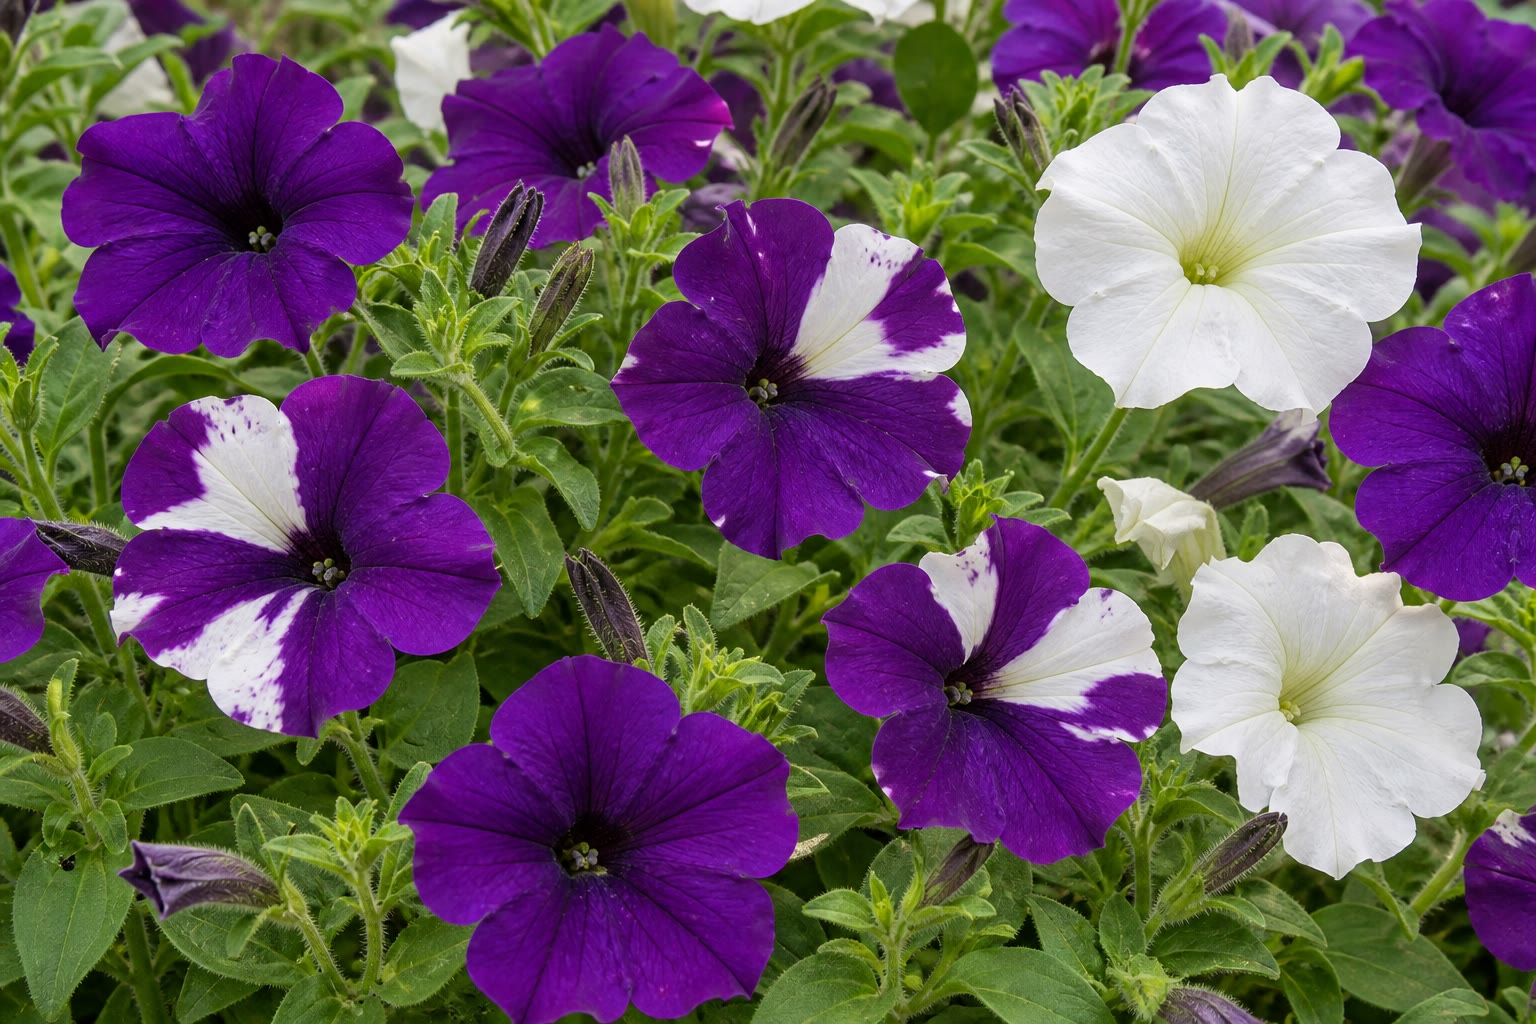
\includegraphics[width=0.46\linewidth]{images/book5/ai/b5-02-petunia-cosuppression.jpg}\hspace{0.04\linewidth}
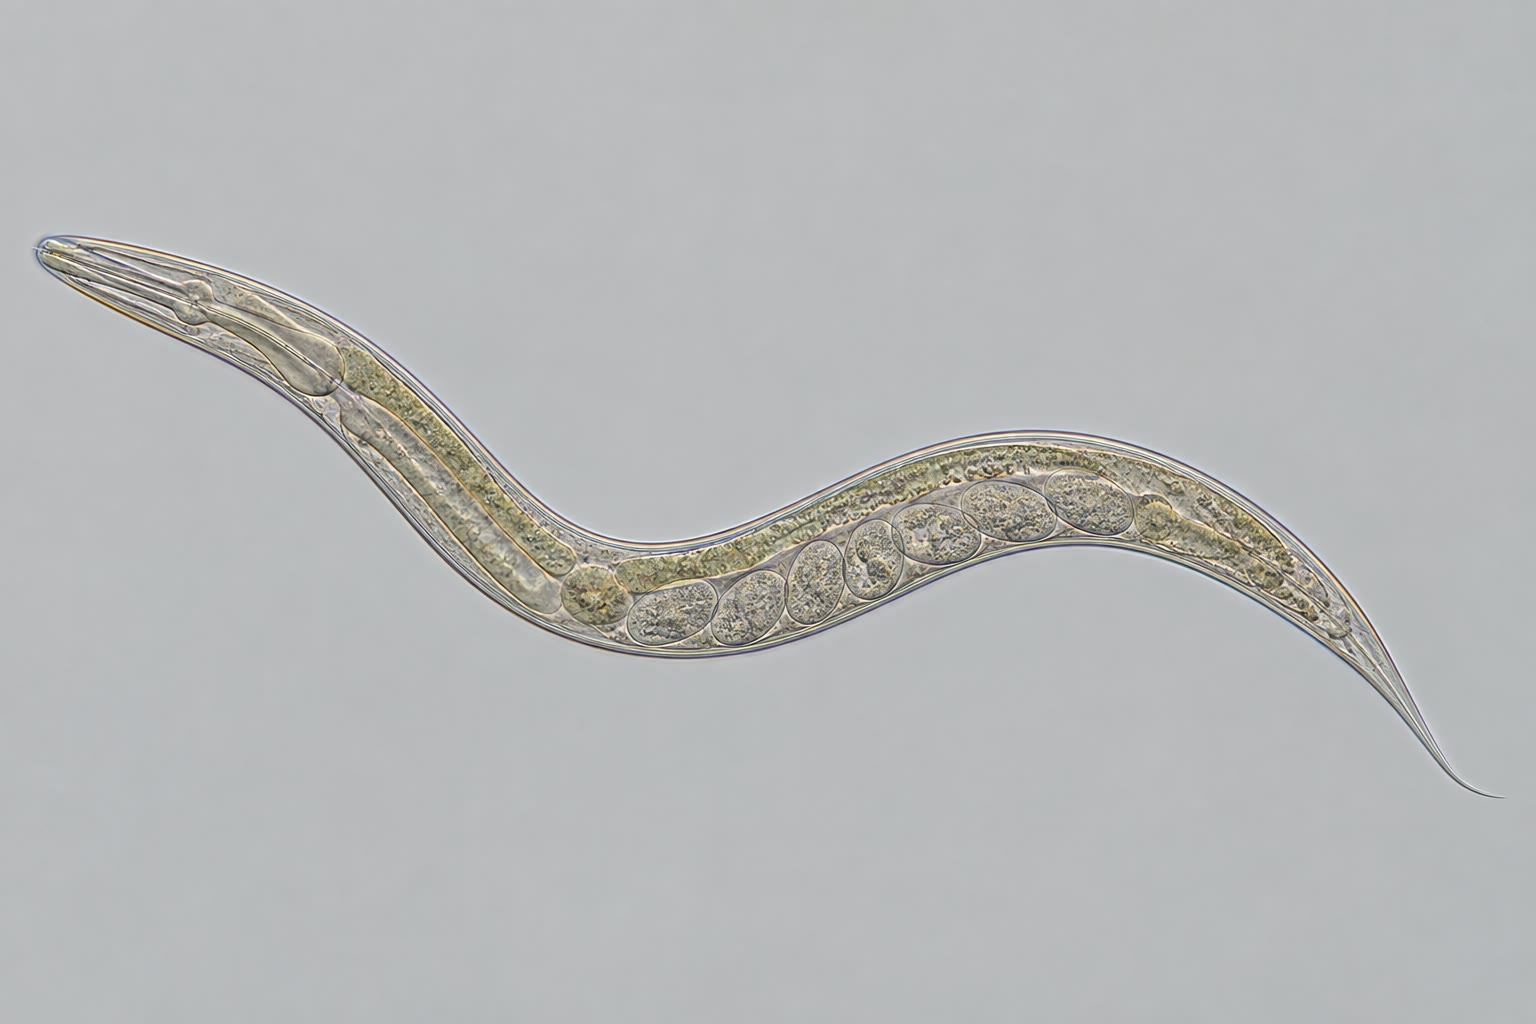
\includegraphics[width=0.46\linewidth]{images/book5/ai/b5-02-c-elegans.jpg}

{\small Links: petunia's met een extra pigmentgen, met de witte
sectoren van cosuppressie. Rechts: de nematode \emph{Caenorhabditis
elegans}, ongeveer een millimeter lang en doorzichtig, waarin
geïnjecteerd dubbelstrengs RNA het passende gen in het hele dier en in
zijn nageslacht uitschakelde.}
\end{omfigure}

\begin{definition}[MicroRNA's]\label{def:b3:rna-regulation:mirna}
\index{microRNA!biogenese}\index{Drosha}\index{seedsequentie}
Een \emph{\omterm{def:b3:rna-regulation:ncrna}{microRNA}} is in het genoom gecodeerd --- in een eigen gen of
in een intron van een eiwitcoderend gen --- en wordt door
RNA-polymerase II afgeschreven als een lang primair transcript
(pri-miRNA) met een haarspeld van ongeveer \qty{70}{nt}. In de kern
knipt het RNase III \emph{Drosha}, met zijn partner DGCR8, de
haarspeld eruit (het pre-miRNA); exportine-5 brengt haar naar het
cytoplasma, waar \omterm{def:b3:rna-regulation:rnai}{Dicer} de lus verwijdert en een duplex van
\qty{22}{nt} overblijft. Eén streng wordt in \omterm{def:b3:rna-regulation:rnai}{Argonaute} geladen. Het
rijpe miRNA herkent zijn doelwitten vooral via zijn \emph{seed}, de
nucleotiden 2 tot 8, die paart met plaatsen die meestal in de
3$'$-niet-vertaalde regio van een boodschapper liggen; de rest van het
miRNA paart onvolledig, zodat het doelwit niet wordt geknipt maar
onderdrukt: het \omterm{def:b3:rna-regulation:rnai}{RISC} trekt eiwitten aan die de poly(A)-staart
inkorten, de kap verwijderen en de translatie remmen, en de
boodschapper wordt sneller afgebroken. Omdat een seed maar zeven
nucleotiden telt, heeft één miRNA honderden doelwitten, en meer dan de
helft van de menselijke eiwitcoderende genen draagt geconserveerde
plaatsen voor minstens één van de enkele honderden zeker
geïdentificeerde menselijke miRNA's.
\end{definition}

\begin{proof}[Bewijsmateriaal]
\emph{lin-4}, een gen dat de worm nodig heeft om van zijn eerste
larvale stadium naar het tweede te gaan, bleek bij Lee, Feinbaum en
Ambros (1993) niet voor een eiwit te coderen maar voor een RNA van
\qty{22}{nt}, complementair aan zeven plaatsen in de
3$'$-niet-vertaalde regio van de boodschapper van \emph{lin-14}, het
gen waarvan bekend was dat het het onderdrukte. Wanneer de larve het
tweede stadium ingaat verdwijnt het LIN-14-eiwit terwijl zijn mRNA
blijft: de onderdrukking is posttranscriptioneel. Reinhart en
collega's (2000) vonden een tweede zo'n RNA, \emph{let-7}, dat de
latere larvale overgangen stuurt; Pasquinelli (2000) vond
\emph{let-7} bij vliegen en mensen, met dezelfde sequentie, en dat
maakte van een wormcuriositeit een algemeen mechanisme.
\end{proof}

\begin{omfigure}
\begin{tikzpicture}[every node/.style={font=\scriptsize}, >=stealth]
  % nucleus box
  \draw[rounded corners=8pt, thick, gray!60, fill=gray!6] (-0.4,-1.1) rectangle (5.2,2.7);
  \node[gray, anchor=south west] at (-0.3,-1.05) {kern};
  % gene and pri-miRNA
  \draw[very thick, omDef] (0,2.0) -- (2.4,2.0); \node[above] at (1.2,2.05) {miRNA-gen, Pol II};
  \draw[->, thick] (1.2,1.85) -- (1.2,1.35);
  % hairpin
  \draw[thick, omThm!70!black] (0.2,1.0) -- (0.9,1.0) .. controls (1.0,1.0) and (1.05,0.9) .. (1.1,0.5) .. controls (1.15,0.1) and (1.25,0.1) .. (1.3,0.5) .. controls (1.35,0.9) and (1.4,1.0) .. (1.5,1.0) -- (2.2,1.0);
  \draw[thick, omThm!70!black] (1.1,0.5) -- (1.3,0.5);
  \node[below] at (1.2,0.0) {pri-miRNA-haarspeld};
  % Drosha
  \draw[thick, fill=omExo!35] (2.9,0.7) ellipse (0.55 and 0.28); \node at (2.9,0.7) {Drosha};
  \draw[->, thick] (2.3,0.85) -- (2.4,0.75);
  \draw[->, thick] (3.5,0.7) -- (4.2,0.7) node[midway, above] {knip};
  % pre-miRNA
  \draw[thick, omThm!70!black] (4.3,0.9) .. controls (4.5,0.9) and (4.55,0.4) .. (4.6,0.1) .. controls (4.65,-0.2) and (4.75,-0.2) .. (4.8,0.1) .. controls (4.85,0.4) and (4.9,0.9) .. (5.1,0.9);
  \node[below, align=center] at (4.7,-0.25) {pre-miRNA\\\qty{70}{nt}};
  % export
  \draw[->, thick] (5.35,0.4) -- (6.3,0.4) node[midway, above, xshift=0.2cm] {exportine-5};
  % cytoplasm
  \node[gray, anchor=north west] at (5.5,2.65) {cytoplasma};
  \draw[thick, fill=omExo!35] (6.9,0.4) ellipse (0.5 and 0.28); \node at (6.9,0.4) {Dicer};
  \draw[->, thick] (7.45,0.4) -- (8.1,0.4);
  \draw[thick, omThm!70!black] (8.2,0.55) -- (9.6,0.55); \draw[thick, omThm!70!black] (8.35,0.25) -- (9.75,0.25);
  \node[below, align=center] at (8.95,0.15) {duplex van \qty{22}{nt}};
  \draw[->, thick] (8.95,-0.4) -- (8.95,-0.9) node[midway, right] {één streng geladen};
  % RISC on mRNA
  \draw[thick, fill=omProp!35] (8.95,-1.45) ellipse (0.85 and 0.35); \node at (8.95,-1.45) {Argonaute};
  \draw[thick, omThm!70!black] (8.3,-1.85) -- (9.6,-1.85);
  \draw[very thick, omDef] (5.6,-2.15) -- (11.4,-2.15);
  \node[below] at (6.4,-2.2) {mRNA: coderende regio}; \node[below] at (10.3,-2.2) {3$'$ UTR, doelplaats};
  \draw[omDef, thick] (11.4,-2.15) -- (11.8,-2.15) node[right] {AAAA};
  \draw[->, thick, omThm] (9.9,-1.5) -- (10.9,-1.5) node[right, align=left] {deadenylering,\\afbraak, minder\\translatie};
  \node[below, align=center] at (8.95,-2.7) {de seed (nt 2--8) paart\\met de plaats};
\end{tikzpicture}

{\small Biogenese van een \omterm{def:b3:rna-regulation:ncrna}{microRNA}. De haarspeld wordt in de kern door
\omterm{def:b3:rna-regulation:mirna}{Drosha} uit het primaire transcript geknipt, geëxporteerd, door \omterm{def:b3:rna-regulation:rnai}{Dicer}
bijgesneden tot een duplex van \qty{22}{nt}, en één streng wordt in
\omterm{def:b3:rna-regulation:rnai}{Argonaute} geladen. De seed paart met een plaats in de
3$'$-niet-vertaalde regio van een boodschapper, en de boodschapper
wordt gedeadenyleerd, afgebroken en minder vertaald.}
\end{omfigure}

\begin{theorem}[Wat een microRNA doet met het niveau en de snelheid van een boodschapper]\label{thm:b3:rna-regulation:mirna-kinetics}
\index{halveringstijd van mRNA}\index{responstijd}
Een boodschapper wordt met constante snelheid $k$ gemaakt en met
eerste-ordesnelheid $\gamma$ afgebroken; een \omterm{def:b3:rna-regulation:ncrna}{microRNA} op niveau $R$
voegt een afbraakterm $\gamma' R\, m$ toe. Dan voldoet het mRNA-niveau
$m(t)$ aan
\[
\frac{\mathrm{d}m}{\mathrm{d}t} = k - (\gamma + \gamma' R)\, m,
\qquad
m^{*} = \frac{k}{\gamma + \gamma' R},
\qquad
m(t) = m^{*} + (m_{0} - m^{*})\,e^{-(\gamma + \gamma' R)t}.
\]
Het \omterm{def:b3:rna-regulation:ncrna}{microRNA} verlaagt de evenwichtstoestand met de factor $1 + \gamma' R/
\gamma$ en verkort de tijdconstante van elke verandering in $m$ met
diezelfde factor, van $1/\gamma$ tot $1/(\gamma + \gamma' R)$. Een gen
onder microRNA-sturing is daarom zowel stiller als sneller: het
bereikt na een verandering van zijn promotor eerder een nieuwe
evenwichtstoestand, en schommelingen in zijn transcriptie worden
gedempt.
\end{theorem}
\begin{proof}
De vergelijking is lineair met constante coëfficiënten; haar vaste punt
is $m^{*}$, waar het rechterlid verdwijnt, en met $u = m - m^{*}$ komt
er $\mathrm{d}u/\mathrm{d}t = -(\gamma + \gamma' R)\,u$, vanwaar de
exponentiële vorm. De halveringstijd van de nadering is $\ln 2/(\gamma + \gamma'
R)$, en $\gamma = \ln 2 / t_{1/2}$ met $t_{1/2}$ de natuurlijke
halveringstijd van de boodschapper.
\end{proof}

\begin{example}[Een viervoudige onderdrukking]\label{ex:b3:rna-regulation:fourfold}
Een boodschapper met een natuurlijke halveringstijd van \qty{30}{min} ($\gamma =
\qty{0.023}{min^{-1}}$), afgeschreven met $k = 2$ moleculen per minuut,
staat op $m^{*} = 2/0.023 \approx 87$ kopieën per cel en heeft
\qty{30}{min} nodig om na een verandering van zijn promotor halverwege
een nieuw niveau te komen. Een \omterm{def:b3:rna-regulation:ncrna}{microRNA} dat zijn afbraaksnelheid
verdrievoudigt ($\gamma' R = 3\gamma$) brengt hem op $22$ kopieën en
snijdt de halveringstijd terug tot \qty{7.5}{min}. Dezelfde getallen,
achterstevoren gelezen, laten zien waarom uitschakeling van een miRNA
vaak milde fenotypen geeft: een viervoudige verandering in een
boodschapper die stroomafwaarts zelf gebufferd is kan het organisme
bijna normaal laten, en het effect komt onder stress of in de timing
naar voren.
\end{example}

\begin{omfigure}
\begin{tikzpicture}
\begin{axis}[
  width=0.7\linewidth, height=5.6cm,
  axis x line=bottom, axis y line=left,
  xmin=0, xmax=120, ymin=0, ymax=100,
  xlabel={tijd nadat de promotor aangaat (min)}, ylabel={mRNA per cel},
  xlabel style={font=\small, at={(axis description cs:0.5,-0.12)}, anchor=north},
  ylabel style={font=\small},
  tick label style={font=\small}, xtick={0,30,60,90,120}, ytick={0,22,50,87},
  clip=false,
]
\addplot[very thick, omDef, domain=0:120, samples=80] {87*(1-exp(-0.0231*x))};
\addplot[very thick, omThm, domain=0:120, samples=80] {21.7*(1-exp(-0.0924*x))};
\addplot[dashed, gray, domain=0:120, samples=2] {87};
\addplot[dashed, gray, domain=0:120, samples=2] {21.7};
\node[font=\scriptsize, omDef, anchor=south west] at (axis cs:5,90) {zonder microRNA: $m^{*} = 87$, halveringstijd \qty{30}{min}};
\node[font=\scriptsize, omThm, anchor=south west] at (axis cs:40,24) {met microRNA, $\gamma' R = 3\gamma$: $m^{*} = 22$, halveringstijd \qty{7.5}{min}};
\end{axis}
\end{tikzpicture}

{\small Stijging van een boodschapper nadat zijn promotor is
aangezet, met de getallen van \cref{ex:b3:rna-regulation:fourfold}.
Het \omterm{def:b3:rna-regulation:ncrna}{microRNA} verlaagt het plateau viervoudig en bereikt het vier keer
zo snel.}
\end{omfigure}

\begin{method}[Een gen uitschakelen met RNAi]\label{met:b3:rna-regulation:knockdown}
\index{knockdown}\index{shRNA}
Om een gen uit te schakelen zonder zijn DNA aan te raken: (1) kies een
sequentie van \qty{21}{nt} die uniek is voor zijn boodschapper en
vermijd seedovereenkomsten met andere genen; (2) lever haar aan als
synthetische siRNA-duplex (tijdelijk, enkele dagen) of als een kort
haarspeld-RNA (shRNA) dat vanuit een vector tot expressie komt en dat
\omterm{def:b3:rna-regulation:rnai}{Dicer} doorlopend verwerkt; voeder wormen bacteriën die het
dubbelstrengs RNA tot expressie brengen; (3) meet de boodschapper met
kwantitatieve PCR en het eiwit met een immunoblot, en verwacht
\qtyrange{70}{95}{\%} verlies in plaats van de volledige afwezigheid
van een knockout; (4) controleer op effecten buiten het doelwit met
een tweede, niet-overlappend \omterm{def:b3:rna-regulation:ncrna}{siRNA} en met een redding door een
RNAi-bestendige versie van het gen. Een knockdown is een gedeeltelijk,
omkeerbaar functieverlies; de gentherapieën die op dit beginsel zijn
goedgekeurd leveren \omterm{def:b3:rna-regulation:ncrna}{siRNA's} tegen boodschappers van de lever
(transthyretine, PCSK9), gekoppeld aan een suiker die de hepatocyt
opneemt.
\end{method}

\section{Kleine RNA's die het genoom bewaken}

\begin{definition}[piRNA's en het uitschakelen van transposons]\label{def:b3:rna-regulation:pirna}
\index{piRNA!ping-pong}\index{uitschakeling van transposons}\index{hybride dysgenese}
\emph{piRNA's} zijn RNA's van \numrange{26}{31} nucleotiden, gemaakt
zonder \omterm{def:b3:rna-regulation:rnai}{Dicer} uit lange enkelstrengs transcripten van genomische
\emph{piRNA-clusters} --- kerkhoven van defecte transposonkopieën ---
en geladen in de PIWI-onderfamilie van de Argonaute-eiwitten in de
kiembaan. Een piRNA dat antisense is aan een transposon stuurt de knip
van de transcripten van dat transposon; het geknipte fragment wordt een
nieuw sense-piRNA, dat op zijn beurt clustertranscripten knipt om meer
antisense-piRNA's te maken --- de \emph{ping-pongcyclus}, een
versterking die zich richt op het transposon dat op dat moment actief
is. Nucleaire PIWI-eiwitten sturen ook H3K9-methylering en
\omterm{def:b3:chromatin-epigenetics:methylation}{DNA-methylering} naar de genomische kopieën van het transposon, wat het
RNA verbindt met de chromatinemerktekens van
\cref{ch:b3:chromatin-epigenetics}. Een moeder legt haar piRNA's in de
eicel; een vrouwtje uit een lijn die nooit een bepaald transposon heeft
ontmoet heeft er geen piRNA's tegen, en haar nakomelingen van een
mannetje dat het draagt zijn steriel --- \emph{hybride dysgenese}, voor
het eerst gezien bij kruisingen van \emph{Drosophila} tussen
laboratorium- en wilde stammen.
\end{definition}

\begin{proposition}[RNA-gestuurde uitschakeling via chromatine]\label{prop:b3:rna-regulation:rddm}
\index{RNA-gestuurde DNA-methylering}
Bij planten methyleert een eigen route --- RNA-polymerase IV schrijft
een locus af, een RNA-afhankelijk RNA-polymerase maakt het transcript
dubbelstrengs, een \omterm{def:b3:rna-regulation:rnai}{Dicer} knipt \omterm{def:b3:rna-regulation:ncrna}{siRNA's} van \qty{24}{nt},
\omterm{def:b3:rna-regulation:rnai}{Argonaute}~4 brengt ze terug naar de ontluikende transcripten van
polymerase V op dezelfde locus en trekt het methyltransferase DRM2 aan
--- het DNA van transposons en herhaalde sequenties; zij is het
mechanisme van de paramutatie. Bij splijtgist trekken \omterm{def:b3:rna-regulation:ncrna}{siRNA's} uit de
centromere herhalingen het H3K9-methyltransferase aan en bouwen zij
het \omterm{def:b3:chromatin-epigenetics:nucleosome}{heterochromatine} dat het centromeer nodig heeft. In beide gevallen
vindt een RNA door complementariteit een plaats in het genoom en wordt
daar een chromatinemerkteken geschreven: sequentiespecifiek,
zichzelf versterkend en erfelijk door de delingen heen.
\end{proposition}

\section{Het leven van een boodschapper}

\begin{definition}[Gereguleerde splicing]\label{def:b3:rna-regulation:splicing}
\index{alternatieve splicing!regulatie}\index{SR-eiwit}\index{hnRNP}\index{overslaan van een exon}
Alternatieve splicing maakt uit één gen verschillende boodschappers
door het \emph{overslaan van een exon}, de keuze tussen elkaar
uitsluitende exons, het behoud van een intron, of het gebruik van
andere 5$'$- of 3$'$-splitsplaatsen. Zij wordt gereguleerd door
RNA-bindende eiwitten die sequentie-elementen binden in de exons en
introns bij een splitsplaats: \emph{SR-eiwitten} gebonden aan
exonische enhancers trekken het spliceosoom aan en bevorderen de
opname van het exon, \emph{hnRNP}-eiwitten gebonden aan silencers
blokkeren haar, en de uitkomst in een gegeven cel wordt bepaald door
de verhouding tussen beide soorten. Meer dan \qty{90}{\%} van de
menselijke genen met meerdere exons wordt alternatief gesplitst; het
\emph{Dscam}-gen van \emph{Drosophila}, met vier blokken elkaar
uitsluitende exons (12, 48, 33 en 2 alternatieven), kan \num{38016}
verschillende eiwitten maken, waarbij elk neuron een andere set tot
expressie brengt die zijn takken elkaar laat herkennen en ontwijken.
\end{definition}

\begin{proof}[Bewijsmateriaal]
Het geslacht van een fruitvlieg wordt beslist door een
splicingcascade. Bij vrouwtjes maakt het gen \emph{Sex-lethal}
(\emph{Sxl}) een werkzaam eiwit; SXL is een RNA-bindend eiwit dat een
splitsplaats blokkeert in zijn eigen transcript (zodat een exon met
een stopcodon wordt overgeslagen en het eiwit gemaakt blijft worden)
en in het transcript van \emph{transformer}, wat de vrouwelijke
splitsing afdwingt; TRA bindt daarna, met TRA-2, een exonische
enhancer in het \emph{doublesex}-transcript en stuurt de vrouwelijke
vorm van de transcriptiefactor DSX. Bij mannetjes, zonder SXL, neemt
elk van deze transcripten de standaardsplitsing, bevat
\emph{transformer} een stopcodon en komt DSX in de mannelijke vorm
uit. Elk geslachtelijk dimorf kenmerk van de vlieg volgt uit welk DSX
wordt gemaakt; een vrouwtje met een mutatie in \emph{tra} ontwikkelt
zich als mannetje.
\end{proof}

\begin{definition}[Stabiliteit en lokalisatie van mRNA]\label{def:b3:rna-regulation:stability}
\index{AU-rijk element}\index{mRNA-lokalisatie}\index{ijzerresponsief element}
De \emph{halveringstijd} van een boodschapper loopt van minuten tot
dagen en wordt bepaald door elementen in zijn 3$'$-niet-vertaalde
regio. \emph{AU-rijke elementen} (AUUUA-herhalingen) in de
boodschappers van cytokinen, groeifactoren en proto-oncogenen worden
gebonden door eiwitten die deadenylasen aantrekken en halveringstijden
van \qtyrange{10}{30}{min} geven, zodat een uitbarsting van
transcriptie een uitbarsting van eiwit oplevert en niet meer dan dat;
mutaties die ze weghalen veroorzaken overexpressie en, voor sommige
proto-oncogenen, kanker. \emph{Lokalisatie-elementen}, vaak met een
structuur, worden gebonden door adaptoren die de boodschapper aan een
motor koppelen: de boodschappers van \emph{bicoid} en \emph{oskar}
worden door dyneïne en kinesine over microtubuli naar de twee polen
van het vliegenei gebracht, de boodschapper van $\beta$-actine naar de
voorrand van een fibroblast, en de boodschappers van synaptische
eiwitten tot in de dendrieten, waar ze op verzoek worden vertaald. Het
\emph{ijzerresponsieve element} (IRE), een steellus die door de
ijzerregulerende eiwitten IRP1 en IRP2 wordt gebonden wanneer ijzer
schaars is, doet vanuit twee posities twee tegengestelde dingen: in de
5$'$-niet-vertaalde regio van de ferritineboodschapper blokkeert
gebonden IRP het ribosoom; in de 3$'$-niet-vertaalde regio van de
boodschapper van de transferrinereceptor beschermt gebonden IRP het
transcript tegen een nuclease.
\end{definition}

\begin{example}[IJzer, gelezen door één haarspeld]\label{ex:b3:rna-regulation:iron}
Bij weinig ijzer bindt IRP beide boodschappers: ferritine, het
opslageiwit, wordt niet vertaald, en de transferrinereceptor, die
ijzer invoert, wordt gestabiliseerd en overvloedig --- de cel slaat
minder op en voert meer in. Bij veel ijzer wordt IRP1 omgezet in een
aconitase (het krijgt een ijzer-zwavelcluster en verliest zijn
affiniteit voor RNA) en wordt de afbraak van IRP2 in gang gezet:
ferritine wordt vertaald, de boodschapper van de receptor vergaat
binnen minuten, en de cel slaat meer op en voert minder in. Er is geen
verandering van transcriptie voor nodig. Een puntmutatie in het IRE
van ferritine die de binding van IRP verhindert veroorzaakt
onophoudelijke ferritinesynthese en het erfelijke
hyperferritinemie-cataractsyndroom.
\end{example}

\begin{omfigure}
\begin{tikzpicture}[every node/.style={font=\scriptsize}, >=stealth]
  \foreach \yy/\state in {2.2/weinig ijzer, -0.9/veel ijzer} {
    \node[left, font=\small\bfseries] at (-0.2,\yy+0.35) {\state};
    % ferritin mRNA
    \draw[very thick, omDef] (0.3,\yy+0.6) -- (4.6,\yy+0.6); \node[below] at (3.3,\yy+0.4) {ferritine-mRNA};
    \draw[thick, omThm!70!black] (0.9,\yy+0.6) .. controls (0.9,\yy+1.15) and (1.3,\yy+1.15) .. (1.3,\yy+0.6); \node[below] at (1.1,\yy+0.55) {IRE};
    \draw[fill=omDef!20, thick] (2.2,\yy+0.42) rectangle (4.4,\yy+0.78);
    % TfR mRNA
    \draw[very thick, omDef] (6.2,\yy+0.6) -- (10.6,\yy+0.6); \node[below, font=\tiny] at (7.1,\yy+0.4) {mRNA van de transferrinereceptor};
    \draw[fill=omDef!20, thick] (6.4,\yy+0.42) rectangle (8.6,\yy+0.78);
    \foreach \x in {9.0,9.5,10.0} \draw[thick, omThm!70!black] (\x,\yy+0.6) .. controls (\x,\yy+1.1) and (\x+0.35,\yy+1.1) .. (\x+0.35,\yy+0.6);
    \node[below, font=\tiny] at (9.9,\yy+0.55) {IRE's (3$'$ UTR)};
  }
  % low iron: IRP bound
  \draw[thick, fill=omProp!40] (1.1,3.35) ellipse (0.4 and 0.24); \node at (1.1,3.35) {IRP};
  \node[right, omThm] at (1.55,3.35) {ribosoom geblokkeerd: geen ferritine};
  \foreach \x in {9.18,9.68,10.18} { \draw[thick, fill=omProp!40] (\x,3.35) ellipse (0.28 and 0.2); }
  \node[above, omMeth!70!black] at (9.7,3.75) {beschermd tegen nuclease: stabiele, overvloedige receptor};
  \node[below, omMeth!70!black] at (1.1,1.75) {slaat minder op};
  \node[below, omMeth!70!black] at (7.4,1.75) {voert meer in};
  % high iron: IRP off
  \node[right, omMeth!70!black] at (1.55,0.25) {vertaald: ferritine gemaakt};
  \node[right, omThm, align=left] at (10.7,-0.3) {nuclease:\\mRNA vergaat};
  \node[below, omThm] at (1.1,-1.35) {slaat meer op};
  \node[below, omThm] at (7.4,-1.35) {voert minder in};
\end{tikzpicture}

{\small Het ijzerresponsieve element. Bij weinig ijzer bindt het
ijzerregulerende eiwit de IRE-haarspelden: aan het 5$'$-uiteinde van
de ferritineboodschapper blokkeert het de translatie, aan het
3$'$-uiteinde van de boodschapper van de transferrinereceptor
blokkeert het een nuclease. Bij veel ijzer laat het eiwit beide los:
ferritine wordt gemaakt, de boodschapper van de receptor vergaat.}
\end{omfigure}

\begin{proposition}[Sturing van de translatie]\label{prop:b3:rna-regulation:translation}
\index{sturing van de translatie}\index{eIF2}\index{riboswitch}\index{stroomopwaarts open leesraam}
De initiatiestap is het gebruikelijke aangrijpingspunt van de \omterm{prop:b3:rna-regulation:translation}{sturing
van de translatie}. Fosforylering van de initiatiefactor \emph{eIF2}
door kinasen die aminozuurgebrek, ongevouwen eiwitten, viraal
dubbelstrengs RNA of haemtekort waarnemen legt de algemene initiatie
binnen minuten stil, met uitzondering van enkele boodschappers met
bijzondere kenmerken --- vooral die met \emph{stroomopwaartse open
leesramen}, korte leesramen in de 5$'$-niet-vertaalde regio die
normaal ribosomen vangen en die onder stress worden overgeslagen,
zodat de stressresponsfactoren (GCN4 bij gist, ATF4 bij zoogdieren)
juist worden gemaakt wanneer al het overige dat niet wordt. De
kapbindende factor eIF4E wordt inactief gehouden door 4E-bindende
eiwitten totdat het groeisignaalkinase mTOR ze fosforyleert: een cel
vertaalt pas op volle snelheid wanneer voedingsstoffen en groeifactoren
dat zeggen. Bij bacteriën doen \emph{riboswitches} het zonder enig
eiwit: een gestructureerde 5$'$-regio bindt een metaboliet
(thiaminepyrofosfaat, S-adenosylmethionine, een purine) en vouwt zich
bij die binding om, waardoor de ribosoombindingsplaats wordt begraven
of een transcriptieterminator ontstaat, zodat een biosynthetisch
operon uitgaat wanneer zijn product overvloedig is.
\end{proposition}

\begin{omfigure}
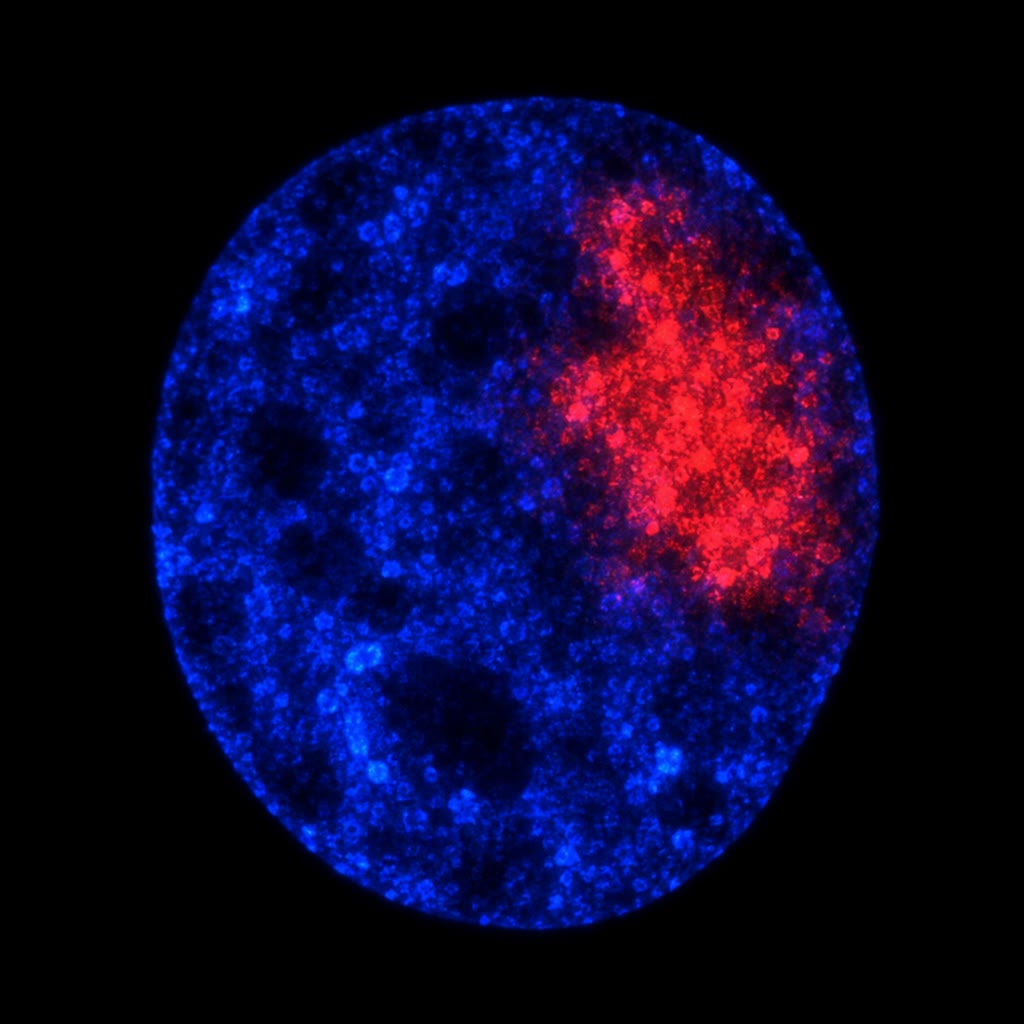
\includegraphics[width=0.36\linewidth]{images/book5/ai/b5-02-lncrna-nucleus.jpg}

{\small Een \omterm{def:b3:rna-regulation:ncrna}{lang niet-coderend RNA} aan het werk: het
\emph{\omterm{def:b3:chromatin-epigenetics:x-inactivation}{Xist}}-transcript (rood), aangetoond met fluorescente
hybridisatie, bekleedt het territorium van één X-chromosoom in een
vrouwelijke kern (DNA in blauw).}
\end{omfigure}

\begin{remark}[Wat posttranscriptionele sturing oplevert]\label{rem:b3:rna-regulation:why}
Transcriptionele sturing werkt via de kern, met een vertraging van
minuten tot uren voordat een nieuwe boodschapper is gemaakt,
uitgevoerd en vertaald. Sturing van de boodschapper zelf werkt daar
waar het eiwit nodig is, in seconden tot minuten, en kan plaatselijk
zijn: één dendriet die één boodschapper bij één synaps vertaalt, de
voorrand van een fibroblast die actine maakt waar hij kruipt. Zij
maakt van één gen ook vele eiwitten, en laat één signaal --- ijzer,
een aminozuur, een \omterm{def:b3:rna-regulation:ncrna}{microRNA} --- honderden boodschappers tegelijk
afstemmen zonder ook maar één promotor aan te raken.
\end{remark}

\section{Opgaven}

\begin{exercise}[$\star$]\label{exo:b3:rna-regulation:1}
Onderscheid miRNA, \omterm{def:b3:rna-regulation:ncrna}{siRNA} en \omterm{def:b3:rna-regulation:pirna}{piRNA} naar herkomst, lengte, afhankelijkheid
van \omterm{def:b3:rna-regulation:rnai}{Dicer}, en wat zij met hun doelwitten doen.
\end{exercise}

\begin{exercise}[$\star$]\label{exo:b3:rna-regulation:2}
Volg de biogenese van een \omterm{def:b3:rna-regulation:ncrna}{microRNA} van zijn gen tot een onderdrukte
boodschapper, en noem bij elke knip het enzym.
\end{exercise}

\begin{exercise}[$\star$]\label{exo:b3:rna-regulation:3}
Waarom schakelde het injecteren van sense-RNA van \emph{unc-22} in
wormen het gen uit in de vroege experimenten, en wat veranderden Fire
en Mello daaraan?
\end{exercise}

\begin{exercise}[$\star$]\label{exo:b3:rna-regulation:4}
Wat gebeurt er met ferritine en met de transferrinereceptor wanneer
een cel van ijzer wordt beroofd? Welke stap van de expressie wordt in
elk van beide gevallen gestuurd?
\end{exercise}

\begin{exercise}[$\star\star$]\label{exo:b3:rna-regulation:5}
Een boodschapper heeft een halveringstijd van \qty{2}{h} en wordt met
$5$ moleculen per minuut gemaakt. Bereken zijn evenwichtsniveau, en
daarna het niveau en de halveringstijd wanneer een \omterm{def:b3:rna-regulation:ncrna}{microRNA} zijn
afbraaksnelheid verdubbelt.
\end{exercise}

\begin{exercise}[$\star\star$]\label{exo:b3:rna-regulation:6}
Een seed van zeven nucleotiden past met kans $4^{-7}$ op een
willekeurige sequentie. Hoeveel plaatsen treft één miRNA-seed bij
toeval in een verzameling van \num{20000} boodschappers met
3$'$-niet-vertaalde regio's van gemiddeld \qty{1000}{nt}? Wat
onderscheidt dan een echt doelwit?
\end{exercise}

\begin{exercise}[$\star\star$]\label{exo:b3:rna-regulation:7}
Voorspel het geslacht van een vlieg (a) met een functieverliesmutatie
in \emph{tra} en twee X-chromosomen; (b) die TRA tot expressie brengt
vanaf een constitutief transgen, met één X; (c) die \emph{dsx} geheel
mist.
\end{exercise}

\begin{exercise}[$\star\star$]\label{exo:b3:rna-regulation:8}
De boodschapper van een proto-oncogen heeft door een \omterm{def:b3:rna-regulation:stability}{AU-rijk element}
normaal een halveringstijd van \qty{15}{min}. Een chromosomale
translocatie haalt het element weg en de halveringstijd wordt
\qty{3}{h}. Met welke factor stijgt het eiwitniveau, als translatie en
eiwitafbraak onveranderd blijven? Waarom is dit oncogeen hoewel het
eiwit normaal is?
\end{exercise}

\begin{exercise}[$\star\star$]\label{exo:b3:rna-regulation:9}
Een laboratoriumstam van \emph{Drosophila} mist P-elementen; een wilde
stam draagt ze. Voorspel de vruchtbaarheid van het nageslacht van
(a) laboratoriumvrouwtjes $\times$ wilde mannetjes, (b) wilde
vrouwtjes $\times$ laboratoriummannetjes, en verklaar de asymmetrie
met \omterm{def:b3:rna-regulation:pirna}{piRNA's}.
\end{exercise}

\begin{exercise}[$\star\star\star$]\label{exo:b3:rna-regulation:10}
Beredeneer met \cref{thm:b3:rna-regulation:mirna-kinetics} dat het
eiwit dat uit een boodschapper wordt gemaakt relatief minder schommelt
wanneer de boodschapper onder microRNA-sturing staat, bij een gelijk
gemiddeld boodschapperniveau. (Het eiwit middelt de boodschapper over
zijn eigen levensduur, en de boodschapper vernieuwt zichzelf sneller.)
Waarom zou een cel voor een \omterm{def:b3:rna-regulation:ncrna}{microRNA} en een hogere transcriptiesnelheid
betalen om hetzelfde gemiddelde te krijgen?
\end{exercise}

\begin{exercise}[$\star\star\star$]\label{exo:b3:rna-regulation:11}
Bij wormen maakt een RNA-afhankelijk RNA-polymerase secundaire \omterm{def:b3:rna-regulation:ncrna}{siRNA's}
uit de doelboodschapper; bij zoogdieren bestaat zo'n polymerase niet.
Voorspel voor elk of uitschakeling door één injectie van dubbelstrengs
RNA vele celdelingen lang standhoudt en of zij zich naar andere
weefsels verspreidt, en verklaar het medische gevolg voor
siRNA-geneesmiddelen.
\end{exercise}

\begin{exercise}[$\star\star\star$]\label{exo:b3:rna-regulation:12}
Een nieuw geannoteerd lncRNA komt in het hart tot expressie. Ontwerp de
experimenten die onderscheid maken tussen (a) een functioneel RNA, (b)
een functionele daad van transcriptie waarvan het RNA er niet toe doet,
en (c) ruis, en zeg welke uitkomst elk daarvan voorspelt.
\end{exercise}

\section{Vraagstuk: de tijdklok van een worm}

\begin{problem}[{Weekendvraagstuk --- de schakelaar
\emph{lin-4}/\emph{lin-14} van de worm getimed met de kinetiek van de
boodschapper, een geïnjecteerd RNA verdund door de delingen van een
embryo en gered door versterking, het ijzerregulon gekwantificeerd en
een telling van splitsvormen, met als besluit de onderdrukkingsfactor,
de halveringstijd van de schakelaar en het aantal delingen dat een
onversterkt signaal overleeft}]
\label{pb:b3:rna-regulation:1}
Gegevens: de boodschapper van \emph{lin-14} wordt met $k = 3$ moleculen
per minuut per cel gemaakt en heeft een halveringstijd van
\qty{40}{min}. Het LIN-14-eiwit wordt met $\beta = 2$ per boodschapper
per minuut gemaakt en heeft een halveringstijd van \qty{3}{h}. Vanaf
het begin van het tweede larvale stadium hoopt het RNA van
\emph{lin-4} zich op en voegt het een afbraakterm $\gamma' R = 3\gamma$
aan de boodschapper toe en halveert het, door de initiatie te
blokkeren, $\beta$. Een wormembryo ontwikkelt zich van één cel tot
ongeveer \num{550} cellen bij het uitkomen; een volwassen dier heeft
\num{959} somatische cellen.

\medskip
\noindent\textbf{Deel I --- De boodschapper.}
\begin{enumerate}
  \item Bereken $\gamma$ en het evenwichtsniveau van de boodschapper
        van \emph{lin-14} voordat \emph{lin-4} verschijnt.
  \item Bereken de afbraaksnelheid van het eiwit en het
        evenwichtsniveau van het LIN-14-eiwit.
  \item Bereken, zodra \emph{lin-4} aanwezig is, het nieuwe niveau van
        de boodschapper en de nieuwe tijdconstante van de boodschapper.
  \item Bereken de nieuwe evenwichtstoestand van het eiwit en de
        onderdrukkingsfactor op het eiwit in het geheel.
  \item Hoe lang na het verschijnen van \emph{lin-4} komt de
        boodschapper halverwege zijn nieuwe niveau? En het eiwit ---
        welke stap begrenst de snelheid van de schakelaar?
  \item De oorspronkelijke experimenten vonden het eiwit verdwenen
        terwijl het mRNA nog aantoonbaar was. Strookt dat met deze
        getallen? Welk deel van de boodschapper blijft over?
\end{enumerate}

\medskip
\noindent\textbf{Deel II --- Verdunning en versterking.}
\begin{enumerate}[resume]
  \item In de gonade van een worm worden $10^{6}$ moleculen
        dubbelstrengs RNA gespoten, die gelijkelijk over \num{250}
        eicellen worden verdeeld. Hoeveel moleculen per eicel?
  \item Als de moleculen bij elke deling eenvoudig zouden worden
        verdeeld, hoeveel zou elke cel van de uitgekomen larve van
        \num{550} cellen er dan bevatten? Na hoeveel verdere delingen
        zou het gemiddelde onder één per cel zakken?
  \item Fire en Mello zagen uitschakeling in het hele dier en in zijn
        nageslacht, bij enkele moleculen per cel. Leg uit wat een
        RNA-afhankelijk RNA-polymerase aan de verklaring toevoegt, en
        waarom het effect toch na enkele generaties uitdooft.
  \item In een zoogdiercel zonder zo'n polymerase brengt een
        siRNA-transfectie \num{5000} duplexen in een cel die zich
        dagelijks deelt; het \omterm{def:b3:rna-regulation:rnai}{RISC} is stabiel maar wordt door de
        deling verdund. Na hoeveel dagen zakt het aantal onder
        \num{100}, ruwweg het aantal dat voor doeltreffende
        uitschakeling nodig is?
  \item Een therapeutisch \omterm{def:b3:rna-regulation:ncrna}{siRNA} tegen een boodschapper van de lever
        wordt eenmaal gegeven en werkt zes maanden. Hepatocyten delen
        zelden. Leg uit waarom het mechanisme van vraag 10 het niet
        begrenst, en wat dat wel doet.
  \item Een seed van zeven nucleotiden past bij toeval eens per
        $4^{7}$ nucleotiden. Het transcriptoom van de worm telt
        ongeveer \qty{20}{Mb} aan 3$'$-niet-vertaalde sequentie.
        Hoeveel toevallige seedovereenkomsten heeft \emph{lin-4}, en
        hoe wisten de genetici welk doelwit ertoe deed?
\end{enumerate}

\medskip
\noindent\textbf{Deel III --- Het ijzerregulon.}
\begin{enumerate}[resume]
  \item In ijzerrijke cellen heeft de boodschapper van de
        transferrinereceptor een halveringstijd van \qty{10}{min}; met
        IRP gebonden \qty{50}{min}. Met welke factor stijgt de
        boodschapper bij onveranderde transcriptie wanneer ijzer
        schaars wordt?
  \item Het niveau van de ferritineboodschapper verandert niet, maar
        haar translatie daalt van $1$ naar $0.05$ eiwitten per
        boodschapper per minuut wanneer IRP bindt. Met welke factor
        daalt de ferritinesynthese?
  \item Combineer beide: met welke factor verandert de verhouding
        tussen invoercapaciteit en opslagcapaciteit tussen de
        ijzerrijke en de ijzerarme toestand?
  \item Het IRP1-eiwit is ofwel een RNA-bindend eiwit ofwel een
        aconitase, afhankelijk van de vraag of het een
        ijzer-zwavelcluster draagt. Leg uit waarom het daardoor een
        sensor van ijzer zelf is en niet van een hormoon.
  \item Een patiënt draagt een IRE-mutatie in ferritine die de binding
        van IRP opheft. Voorspel het ferritineniveau, het serumijzer,
        en waarom de ooglens is aangedaan.
  \item Leg in één zin uit waarom dezelfde haarspeld op de ene positie
        kan activeren en op de andere kan onderdrukken.
  \item IRP2 heeft geen ijzer-zwavelcluster; bij veel ijzer wordt het
        vernietigd door een ubiquitineligase waarvan de eigen
        stabiliteit ijzer en zuurstof vereist. Waarom zou een cel twee
        sensoren met zo verschillende chemie aanhouden?
\end{enumerate}

\medskip
\noindent\textbf{Deel IV --- Splitsvormen tellen.}
\begin{enumerate}[resume]
  \item \emph{Dscam} heeft exonblokken met 12, 48, 33 en 2 elkaar
        uitsluitende alternatieven. Hoeveel splitsvormen? Als elk
        neuron er ongeveer $50$ willekeurig tot expressie brengt, wat
        is dan de kans dat twee gegeven neuronen er minstens één
        delen? (Gebruik $1 - (1 -
        50/N)^{50}$.)
  \item Waarom heeft een neuron er baat bij splitsvormen te hebben die
        zijn buren vrijwel zeker missen?
  \item Hoeveel boodschappers geeft een gen met $n$ cassette-exons die
        elk onafhankelijk worden opgenomen of overgeslagen? Hoeveel
        voor $n = 10$? Waarom is het werkelijke aantal in een gegeven
        celtype meestal veel kleiner?
  \item Waarom sterft bij de vlieg een vrouwtje met twee X-chromosomen
        maar een nulallel van \emph{Sxl}, in plaats van zich eenvoudig
        als mannetje te ontwikkelen? (Bedenk wat het X-telsysteem nog
        meer stuurt: de \omterm{def:b3:chromatin-epigenetics:x-inactivation}{dosiscompensatie} van X-gebonden genen.)
  \item SXL bevordert de productieve splitsing van zijn eigen
        transcript. Leg uit waarom de geslachtsbeslissing daardoor een
        geheugen wordt dat standhoudt nadat het X-telsignaal, dat
        alleen in het vroege embryo aanwezig is, is verdwenen, en
        verbind dit met de zichzelf onderhoudende schakelaars van
        \cref{ch:b3:chromatin-epigenetics}.
  \item Vat de tijdklok samen: de onderdrukkingsfactor op het
        LIN-14-eiwit (vraag~4), de halveringstijd van de schakelaar van
        de boodschapper (vraag~5) en het aantal delingen dat een
        onversterkt signaal overleeft voordat het onder één molecuul
        per cel zakt (vraag~8).
\end{enumerate}
\end{problem}
